\chapter{Rejecting Hallucinations: Addressing Delusional Planning Behaviors}
\label{cha:delusions}
% {\small
% Some materials of this chapter had been used to form \citet{zhao2024delusions}, which was published as a short-form conference paper in International Conference on Machine Learning (ICML), 2025. % \textit{Following the McGill's guidelines on traditional thesis, this chapter is NOT in the form of a manuscript and focuses on the complete presentation of methodology and findings of the corresponding thesis research milestone, which is different from \citet{zhao2024delusions}. Comprehensive discussions of contributions, limitations, encompassing all methodologies and findings of all thesis milestones will be conducted in Chap.~\ref{cha:conclusion}.}
% }

\minitoc

\section{Overview of This Thesis Milestone}
\label{sec:delusions_intro}

\textit{In planning processes of computational decision-making agents, generative or predictive models are often used as ``generators'' to propose ``targets'' representing sets of expected or desirable states. Unfortunately, learned models inevitably hallucinate infeasible targets that can cause delusional behaviors and safety concerns. We first investigate the kinds of infeasible targets that generators can hallucinate. Then, we devise a strategy to identify and reject infeasible targets by learning a target feasibility evaluator. To ensure that the evaluator is robust and non-delusional, we adopted a design choice combining off-policy compatible learning rule, distributional architecture, and data augmentation based on hindsight relabeling. Attaching to a planning agent, the designed evaluator learns by observing the agent's interactions with the environment and the targets produced by its generator, without the need to change the agent or its generator. Our controlled experiments show significant reductions in delusional behaviors and performance improvements for various kinds of existing agents.}

The advent of computational modeling has spurred advancements in computational decision making agents, most notable of which is, model-based RL. This work is focused on those models that play the role of \textit{generators}, which imagine or specify future outcomes for agents. Some generators imagine next states or observations, while others specify subgoals (sets of states) to accomplish. No matter how they are represented, we refer to these generator outputs as \textit{targets} and methods that make such use of generators \textit{Target-Assisted Planning (TAP)}.

TAP is a new perspective for unifying many planning / reasoning agents with wildly different behaviors. For instance, some rollout-based model-based RL methods are TAP, such as those following the classic \Dyna{} or Monte-Carlo tree-search frameworks, utilize fixed-horizon transition models to simulate experiences \citep{sutton1991dyna,schrittwieser2019mastering,kaiser2019model}; While, TAP also encompasses methods that directly generate arbitrarily distant targets acting as candidate sub-goals to divide-and-conquer the tasks into smaller, more manageable steps \citep{zadem2024reconciling,zhao2024consciousness,lo2024goal}.

It is the defining characteristic of TAP - the usage of generators, that brings us to the topic of this work: an often unstated assumption is that generated targets are always feasible. However, the desired generalization abilities of generative models are inevitably accompanied by \textit{hallucinations} \citep{xu2024hallucination,zhang2024generalization,xing2024mitigating,jesson2024estimating,aithal2024understanding} - the ``dark side'' that produces infeasible targets that can never be experienced by anyhow. Hallucinations impact TAP agents differently based on their planning behaviors. In \textit{decision-time} TAP methods ~\citep{alver2022understanding}, where models are used to make an immediate decision on what to do next, hallucinated targets can lead to delusional plans that compromise performance and safety \citep{langosco2022goal,bengio2024managing}. For \textit{background} TAP agents that train on simulated experiences constructed with generated targets, delusional values estimated from hallucinated targets can be catastrophically destabilizing \citep{jafferjee2020hallucinating,lo2024goal}.

\begin{figure}[tbp]
\centering
\includegraphics[width=0.7\textwidth]{figures/Delusions/fig_TAP_framework.pdf}
\caption[Target Evaluator attached to a Target-Assisted Planning (TAP) Agent]{\textbf{Target Evaluator attached to a Target-Assisted Planning (TAP) Agent}:  An abstracted framework that encompasses, but is not limited to, methods listed in Tab.~\ref{tab:methods}. The \textit{generator} proposes candidate target embeddings $\bm{g}^\odot$. Our proposed \textit{evaluator} can be attached to learn to reject infeasible targets (related parts marked in dashed lines).
}
\label{fig:TAP_framework}
\end{figure}

Hallucination and creativity are the two-sides of the same coin that is the generalization ability of the learned models. In psychiatry, it is widely accepted that human brains reject infeasible intentions hallucinated by the belief formation system (that can often hallucinate, similar to the generators in TAP agents) using a belief evaluation system, which acts like a firewall \citep{kiran2009understanding}. Inspired by such discussions, we propose to assist existing TAP agents with a target evaluator, which can be used to reject infeasible targets and in turn delusional behaviors. To maximize compatibility, the evaluator is designed as a minimally-intrusive add-on to attach to existing TAP agents \citet{zhao2020meta}: it learns by observing the TAP agent's interactions with the environment and the targets produced, without the need to change the agent's behaviors or the architecture.. Our main contributions are as follows: 

\begin{enumerate}[leftmargin=*]
\item We systematically categorized and characterized infeasible targets \wrt{} time horizons
\item We discussed the desiderata of learning a minimally-intrusive non-delusional target evaluator
\item We proposed a combination of a) off-policy compatible update rule that enables the evaluator to learn by observing, b) an evaluator architecture compatible with different time horizons that enables a unified solution for most TAP agents and c) two assistive hindsight relabeling strategies performing data augmentation to provide training data beyond those collected via interactions, which ensure that the evaluator itself does not produce delusional evaluations
\item We implemented the solution, as illustrated in Fig.~\ref{fig:TAP_framework}, for several types of existing TAP agents, as discussed in Tab.~\ref{tab:methods}, and showed that agents can better manage generated targets, reduce delusional behaviors and significantly improve performance
\end{enumerate}

\begin{table*}[htbp]
\centering
\aboverulesep=0ex
\belowrulesep=0ex
\caption[Discussed Methods, Properties \& How to use the Feasibility Evaluator]{\textbf{Discussed Methods, Properties \& How to use the Feasibility Evaluator}}
 \resizebox{\textwidth}{!}{
 \begin{NiceTabular}{m[c]{0.1\textwidth}|m[c]{0.16\textwidth}|m[l]{0.3\textwidth}|m[l]{0.35\textwidth}|m[l]{0.4\textwidth}}
 
\toprule

\textbf{Method} & \textbf{TAP Category} & \textbf{Delusional Planning Behaviors} & \textbf{How Our Solution Helps} & \textbf{Implementation Details \& Challenges} \\ \hline
\Dyna{} \citep{sutton1991dyna} & Fixed-Horizon Background Planning & The imagined transitions could contain hallucinated (next) observations / states, whose delusional value estimates could destabilize the bootstrapping-based TD learning & Cancel updates involving rejected next states (not evaluated to be reachable within $1$ timestep). & \cellcolor{blue!25} \textbf{Implemented} (for 1-step Dyna): If the output histogram of the evaluator has significant density on the bin corresponding to $t=1$, then accept the generation, or else, reject \\ \hline
\Dreamer{} \citep{hafner2023mastering} & Fixed-Horizon Background Planning & The imagined trajectories could contain infeasible, hallucinated states & Do not let the rejected imagined states participate in the construction of update targets for the actor-critic system (See Sec.\ref{sec:appendix_dreamer}). & \cellcolor{blue!10} \textbf{Implemented} (insufficient compute for results, Sec.~\ref{sec:appendix_dreamer}): Use the deterministic state $\bm{s}$ as the state representation to feed to the evaluator (also for imagined future target states). Establish $h$ with Mahalanobis distance on the state representations and use the discount, reward and value predictions to force behavioral realism. Truncate $\lambda$-returns until infeasible imagined target states. \\ \hline
\Director{} \citep{hafner2022deep} & Fixed-Horizon Decision-Time Planning (mainly) & The internally sampled goals may be unreachable & Reject unreachable goals and re-sample reachable ones & \cellcolor{blue!10} Similar to our implementation for \Dreamer{}. \\ \hline
\MuZero{} \citep{schrittwieser2019mastering} & Fixed-Horizon Decision-Time Planning & The predicted states in the tree search could be unreachable hallucinations & Reject hallucinated state generations, regenerate node in tree search if necessary & \cellcolor{blue!10} Similar to our implementation for 1-step \Dyna{} \\ \hline
\SimPLe{} \citep{kaiser2019model} & Fixed-Horizon Background Planning & The predicted next observation could be an unreachable hallucination & Reject learning against the delusional estimates (potential) & \cellcolor{blue!10} Similar to our implementation for 1-step \Dyna{} \\ \hline
\Skipper{} \citep{zhao2024consciousness} & Arbitrary-Horizon Decision-Time Planning & Hallucinated subgoals could lead to decision-time planning committing to them, leading to unsafe behaviors & Use an evaluator to learn that the expected cumulative discount is $0$ when aiming to reach the hallucinated subgoals. This disconnects the hallucinated subgoals from the current state in the planning & \cellcolor{green!25} \textbf{Implemented}: diversify the source-target pairs with \generatestr{} and \pertaskstr{} mixtures. $\scriptG{}$ is discrete and $h$ is a trivial comparison. \\ \hline
\GSP{} \citep{lo2024goal} & Arbitrary-Horizon Background Planning & Hallucinated subgoals could lead to value estimation destabilization, like in \Dyna{}. & Use output histogram of the add-on evaluator to correct the delusions by \GSP{}'s own estimators. Use the ``support swap'' technique. & \cellcolor{green!10} Similar to our implementation for \Skipper{} \\ \hline
\LEAP{} \citep{nasiriany2019planning} & Arbitrary-Horizon Decision-Time Planning & Hallucinated subgoals could help fake a sequence of subgoals that is too good to be true and committed to during planning & Use an evaluator to learn that the expected cumulative distance is infinite when aiming to reach the hallucinated subgoals. This makes sure that subgoal sequences containing hallucinated subgoals will not be favored & \cellcolor{red!25} \textbf{Implemented}: pay attention to the representation space of the sub-goals.  \\ \hline
\PlaNet{} \citep{hafner2019learning} & Arbitrary-Horizon Decision-Time Planning & Hallucinated subgoals could help fake a sequence of subgoals that is too good to be true and committed to during planning & Reject the delusional subgoals and therefore reject the delusional subgoal sequences & \cellcolor{red!10} Same as our implementation for \LEAP{} (both uses CEM for planning \citep{rubinstein1997optimization}) \\ \hline
\bottomrule
 \end{NiceTabular}%
 }
\small \textit{Similar colors are used to denote similar implementations for the solution proposed in this work.}

\label{tab:methods}
\end{table*}

\section{Methodology: Target Evaluation \& Relabeling}
\label{sec:delusions_prelim}

\subsection{Target-Assisted Planning \& Targets}
\label{sec:target_directed_framework}
In this work, for generality, we consider a target to be an embedding representing a set of states. Each target $\bm{g}^\odot \mapsto \{ s^\odot \}$ is paired with an indicator function $h$ outputting $h(s',\bm{g}^\odot)=1$ if $s' \in  \{ s^\odot \}$ and $0$ otherwise. For the interest of time horizons, we also introduce $\tau$ - the maximum number of time steps an agent is allowed to reach a state in $\bm{g}^\odot$.

Let $D_\pi(s,\bm{g})$ represents \textit{\nth{1}} timestep $t$ \st{} $h(s_t,\bm{g}^\odot) = 1$, if $\pi$ (conditional or not) is followed from state $s$. We define \textbf{$\tau$-feasibility} of $\bm{g}^\odot$ from state $s$ under $\pi$ as $p(D_\pi(s, \bm{g}^\odot) \leq \tau) \coloneqq \sum_{t=1}^{\tau} p(D_\pi(s, \bm{g}^\odot) = t)$. $\bm{g}^\odot$ is called \textbf{$\tau$-feasible} if $p(D_\pi(s, \bm{g}^\odot) \leq \tau) > 0$, and \textbf{$\tau$-infeasible} otherwise. Notably, $\tau$-feasibility is an intrinsic property of a state-policy-target tuple, not a heuristic measure.

Aligning with the RL objective of maximizing returns, a target is good if it leads to rewarding outcomes, \ie{}:
\begin{align}\label{eq:utility}
\begin{split}
& \scriptU_{\pi, \mu} (s, \bm{g}^\odot, \tau) \coloneqq \\
& r_{\pi}(s, \bm{g}^\odot, \tau) + \gamma_\pi(s, \bm{g}^\odot, \tau) \cdot V_\mu(s_{\min(D_\pi(s,\bm{g}^\odot), \tau)})
% \underbrace{\gamma_{\pi}(s, \bm{g}^\odot | h, \tau)}_\text{``feasibility''} \cdot V_{\mu}(g^\odot|s,\pi,h) \\
\end{split}
\end{align}
where $\min(D_\pi(s,\bm{g}^\odot), \tau)$ denotes the timestep when the commitment to $\bm{g}^\odot$ is terminated (by $h$ or $\tau$), $s_{\min(D_\pi(s,\bm{g}^\odot), \tau)}$ is the state the agent ended up in, $r_{\pi}(s, \bm{g}^\odot, \tau) \coloneqq \sum_{t=1}^{\min(D_\pi(s,\bm{g}^\odot), \tau)}{\gamma^{t-1} r_t}$ is the cumulative discounted reward along the way, $ \gamma_\pi(s, \bm{g}^\odot, \tau) \coloneqq \gamma^{\min(D_\pi(s,\bm{g}^\odot), \tau)}$ is the cumulative discount, and $V_\mu(\cdots)$ is the future value for following $\mu$ afterwards.

Eq.~\ref{eq:utility} shows that if $\bm{g}^\odot$ is $\tau$-infeasible, \ie{}, $s_{min(D_\pi, \tau)} \notin \bm{g}^\odot$, then TAP methods blindly using $\bm{g}^\odot$ to determine $V_\mu$ will produce delusional evaluations - the cause of delusional planning behaviors. For example, feasibility-unaware methods, \eg{}, \citet{sutton1991dyna,schrittwieser2019mastering,hafner2023mastering}, assume that targets are always reachable as long as they can be generated. Meanwhile, planned trajectories involving infeasible targets are delusional; There are also some feasibility-aware methods, \eg{} \citet{nasiriany2019planning,zhao2024consciousness,lo2024goal}, in which agents estimate certain metrics to decide if a target is feasible. However, as we will discuss later, they often produce incorrect estimates, thus may still favor infeasible targets. In later sections, we propose an evaluator that simultaneously estimates the $\tau$-feasibility and $D_\pi$ of the proposed targets, where these estimations are used to decide if the evaluation of a target should be trusted or if the target should be rejected.

\subsection{Source-Target Pairs \& Hindsight Relabeling}

To learn the feasibility of a target from a given state, ``source-target pairs'' are needed, which are tuples involving a source state and a target embedding. The quality of these paired training data is critical for the training outcome \citep{dai2021diversity,moro2022goaldirected,davchev2021wish}. Hindsight Experience Replay (HER) can be seen as a way to enhance the diversity of the pairs, by re-using targets that happened to have been achieved on existing trajectories, and pretending that they were the chosen targets during the interactions \citep{andrychowicz2017hindsight}. \textbf{Relabeling strategies}, corresponding to how $s^{\odot}$ is obtained, are critical for HER's performance \citep{shams2022addressing,eysenbach2021clearning}. Most existing relabeling strategies are \textit{trajectory-level}, meaning that $s^{\odot}$ comes from the same trajectory as $s_t$. These include \futurestr{}, where $s^{\odot} \leftarrow s_{t'}$ with $t' > t$, and \episodestr{}, with $0 \leq t' \leq T_\perp$. HER greatly enhanced the sample efficiency of learning about experienced targets. Meanwhile, its limitations to learning about only experienced targets planted a hidden risk of delusions towards hallucinated targets for TAP agents, to be discussed later. For more discussions regarding Hindsight Experience Replay (HER) and hindsight relabeling strategies, please see Sec.~\ref{sec:source_target_pair_hindsight_relabeling} on Page.~\pageref{sec:source_target_pair_hindsight_relabeling}.

\section{Methodology: Understanding Hallucinated State Targets}
\label{sec:problematic_targets}

Categorizing targets proposed by the generator helps inform us about how to correctly learn the feasibility of targets, \st{} hallucinated targets can be properly rejected.

Let us warm-up with singleton targets, \ie{}, $\bm{g}^\odot$ has a single element $\hat{s}^\odot$, and propose a characterization of singleton targets into $3$ \textit{disjoint} categories, which we call \Gzero{}, \Gone{} and \Gtwo{}. Then, we will extend to the non-singleton targets composed of these $3$ ``ingredients''.

\gdelusion{delusion:g0}
\subsection{\Gzero{}: \texorpdfstring{$\infty$-Feasible}{Feasible}}
Given source state $s$, a generated singleton target $\bm{g}^\odot$ is called \Gzero{} if it maps to one state which is $\infty$-feasible from $s$, with some policy $\pi$. Note that \Gzero{} includes $\tau$-infeasible states for given finite values of $\tau$.

% \Gzero{}s belong to $\scriptS$ of the MDP and are safe for use in planning.

\gdelusion{delusion:g1}
\subsection{\Gone{} - Permanently Infeasible (Hallucinated)}
\Gone{} includes generated ``states'' that do not belong to the MDP at all, \ie{}, a target ``state'' $\hat{s}^\odot$ is \Gone{} if $\forall s,\pi,~ p(D_\pi(s, \hat{s}^\odot) < \infty) = 0$. 

% Note that imperfectly generated targets \textit{corresponding} to valid states can be feasible.

\gdelusion{delusion:g2}
\subsection{\Gtwo{} - Temporarily Infeasible (Hallucinated)}
This type includes those MDP states that are \textit{currently infeasible from state $s$}. Unlike \Gone{}, \Gtwo{} states could be \Gzero{} if they were evaluated from a different source state. \Gtwo{}s can often be overlooked, not only because hallucinations are mostly studied in contexts that do consider the source state $s$, but also because they only exist in some special MDPs.


\subsection{Examples}

To provide intuition about these concepts, we use the MiniGrid platform to create a set of fully-observable environments, minimizing extraneous factors to focus on the targets \citep{chevalierboisvert2023minigrid}. We call this environment \SSMfull{} (\SSM{} for short); In \SSM{}, agents navigate by moving one step at a time in one of four directions across fields of randomly placed, episode-terminating lava-traps, while searching for both a sword and a shield to defeat a monster with a terminal reward. The lava-traps' density is controlled by a difficulty parameter $\delta$, but there is always a feasible path to success. Approaching the monster without both the randomly placed sword and shield ends the episode. Once acquired, either of the two items cannot be dropped, leading to a state space where not all states are accessible from the others. Thus, \SSM{} states are partitioned into $4$ semantic classes, defined by $2$ indicators for sword and shield possession. For example, $\langle 0, 1 \rangle$ denotes ``sword not acquired, shield acquired''.

\Gone{} generations in this environment may be semantically valid, \eg{}, an \SSM{} ``state'' with the agent surrounded by lava, as in Fig.~\ref{fig:example_delusions} (top row), or totally absurd, \eg{}, an \SSM{} observation without an agent.

\begin{figure}[htbp]
\captionsetup[subfigure]{labelformat=empty}
\centering
\subfloat[\Gone{}-induced delusional behavior]{
\captionsetup{justification = centering}
\includegraphics[width=0.238\textwidth]{figures/Delusions/fig_example_delusion_G1E1.pdf}}
\hfill
\subfloat[]{
\captionsetup{justification = centering}
\includegraphics[width=0.23\textwidth]{figures/Delusions/fig_example_delusion_legend.pdf}}
\subfloat[\Gtwo{}-induced delusional behavior ($s$ in $\langle 1, 1 \rangle$, $s^\odot$ in $\langle 0, 0 \rangle$)]{
\captionsetup{justification = centering}
\includegraphics[width=0.48\textwidth]{figures/Delusions/fig_example_delusion_G2E2.pdf}}
\caption[Delusional Plans in SSM]{\textbf{Delusional Plans in \SSM{}}: In both cases, a TAP agent, lacking understanding about the hallucinated targets (yellow dots), mis-evaluates their feasibility, leading to delusional plans which suggest that the task goal can be achieved via the infeasible targets.
}
\label{fig:example_delusions}
\end{figure}

\Gtwo{} states can be once \Gzero{} but are now blocked due to a past transition, \eg{}, after acquiring the sword in \SSM{}, the agent transitions from class $\langle 0, 0\rangle$ to $\langle 1, 0\rangle$, sealing off access to $\langle 0, 0\rangle$ or $\langle 0, 1\rangle$; \Gtwo{} can also appear due to the initial state distribution $d$: some states can only be accessed from specific initial states, \eg{}, an agent spawned in $\langle 1, 0\rangle$ cannot reach $\langle 0, 0\rangle$ or $\langle 0, 1\rangle$. An example of delusional behavior caused by a \Gtwo{} target is provided in Fig.~\ref{fig:example_delusions} (bottom row).

Despite rising concerns regarding the safety of TAP agents \citep{bengio2024managing}, their delusional behaviors remain under-investigated, largely due to the \textbf{lack of access} to ground truths needed to identify hallucinations and their resulting delusional behaviors. Thus, it is critical to analyze with clear examples and conduct rigorous controlled experiments where the ground truth of targets could be solved with Dynamic Programming (DP) \citep{howard1960dynamic}, which is why we created \SSM{} and used it later for experiments.

\subsection{Non-Singleton Targets}

For the general case, where a generated target embedding $\bm{g}^\odot$ potentially corresponds to a set of ``states'' $\{\hat{s}^\odot\}$, the elements of the associated set may span all categories, \ie{}, the target can correspond to a mixture of \Gzero{}, \Gone{} \& \Gtwo{} states. Tab.~\ref{tab:birdseye} summarizes the possible target compositions and their properties\footnote{There may be no explicit mapping from a target embedding to a set of ``states'' and thus any target can always map to arbitrarily many \Gone{} ``states''. Thm.~\ref{thm:feasibility_reduction} explains that this problem is benign.}.

\begin{table*}[htbp]
\centering
\aboverulesep=0ex
\belowrulesep=0ex
\caption[Categorization of Targets based on Composition, Characteristics, Risks \& Delusion Mitigation Strategies]{\textbf{Categorization of Targets based on Composition, Characteristics, Risks \& Delusion Mitigation Strategies}}
 \resizebox{\textwidth}{!}{
 \begin{NiceTabular}{m[c]{0.12\textwidth}|m[l]{0.17\textwidth}|m[c]{0.17\textwidth}|m[l]{0.32\textwidth}|m[l]{0.32\textwidth}}
 
\toprule

\textbf{Target Composition} & \textbf{State Correspondence} & \textbf{$\infty$-Feasibility} $p(D_\pi(s, \bm{g}^\odot) < \infty)$ & \textbf{Feasibility Errors \& Resulting Delusional Planning Behaviors} & \textbf{Data Augmentation (Relabeling) Strategies against Feasibility Delusions} \\
\hline
\textbf{Only or Single \Gzero{}} & non-hallucinated feasible states from $s$ & $>0$ & \edelusion{delusion:e0} \textbf{\Ezero{}}: May think \Gzero{} states are infeasible, thus turn to riskier alternatives, \eg{}, \Gone{} or \Gtwo{} & \episodestr{} for \Gzero{} (and \Gtwo{}) states in the same episode + \pertaskstr{} for \Gzero{} (and \Gtwo{}) beyond the episode \\
\hline
\textbf{Only or Single \Gone{}} & hallucinated ``states'' not belonging to the MDP & should $=0$ & \edelusion{delusion:e1} \textbf{\Eone{}}: May think \Gone{} states are favorable, thus commit to them. Impacted by ill-defined  $V_\mu(\cdots)$ & \generatestr{} for \Gone{} (and \Gzero{} \& \Gtwo{}) states, to be proposed by the generator \\
\hline
\textbf{Only or Single \Gtwo{}} & hallucinated MDP states infeasible from $s$ & should $=0$ & \edelusion{delusion:e2} \textbf{\Etwo{}}: May think \Gtwo{} states are favorable, thus commit to them & \pertaskstr{} for \Gtwo{} (and \Gzero{}) beyond episode + \episodestr{} for \Gtwo{} (and \Gzero{}) states in the same episode \\
\bottomrule
\textbf{Some \Gzero{}} & at least one non-hallucinated state from $s$ & $=$ \newline $p(D_\pi(s, \bm{g}_{-}^\odot) < \infty)$ \newline $>0$ (Thm.~\ref{thm:feasibility_reduction}) & \textbf{\Ezero{}} & \episodestr{} + \pertaskstr{}\\ %  May think \Gzero{} states are infeasible, thus turn to riskier alternatives, \eg{}, \Gone{} or \Gtwo{}
\hline
\textbf{Only \Gone{} \& \Gtwo{}} & set of ONLY hallucinated states & should $=0$ & \textbf{\Eone{}} \& \textbf{\Etwo{}} & \generatestr{} or \generatestr{} + \pertaskstr{} \\
\bottomrule
 \end{NiceTabular}%
 }
% \small \textit{This table presents the structural relationships among the important ideas involved in this work.}

\label{tab:birdseye}
\end{table*}

\section{Methodology: Evaluating Targets Correctly and Robustly}
\label{sec:delusions_solutions}

Knowing that hallucinations cannot be eradicated in general, we intend to lower their risks by adopting the brain-inspired solution - to reject infeasible targets post-generation. If done effectively, the negative impact of hallucinated targets becomes limited to the resource cost of generating and rejecting targets, to be discussed in detail. This approach is in contrast with directly trying to address hallucinations in the generators case-by-case, which we deem to have an unbreakable glass ceiling and not versatile enough to be generalized to generic TAP methods. In contrast, agents without evaluators accept proposed targets unconditionally and thus are at risk of delusional planning behaviors.

For a feasibility evaluator to be effectively differentiate the proposed targets, it should correctly estimate the feasibility of targets which maps to all kinds of states (\Gzero{}, \Gone{} \& \Gtwo{}). However, learning to estimate feasibility is not as trivial as it seems, because improper training could naturally lead to delusional feasibility estimations, which cannot be simply addressed by scaling up training. If the evaluator has delusions of feasibility, then its incorporation becomes futile, as hallucinated targets could still be favored.

For estimation errors, we similarly warm up with those of the singleton targets. For clarity, we use matching identifiers \Ezero{}, \Eone{}, and \Etwo{} to denote the estimation errors of feasibility towards \Gzero{}, \Gone{}, and \Gtwo{} ``states'', respectively. These discussions are presented in Tab.~\ref{tab:birdseye}.

When targets correspond to general sets of states, we have:

\begin{result}
    Let $\bm{g}^\odot$ be a target embedding. Its feasibility from state $s$ satisfies:
    \vspace*{-2mm}
    $$\forall \pi, p(D_\pi(s,\bm{g}^\odot) \leq \tau ) = p(D_\pi(s, \bm{g}_{-}^\odot) \leq \tau )$$
    where $\bm{g}^\odot_{-}$ is a target that correspond to the set of states of $\bm{g}^\odot$ with all infeasible states (\Gone{} \& \Gtwo{}) removed.
    \label{thm:feasibility_reduction}
\end{result}

This result indicates that a target is infeasible if and only if it consists entirely of infeasible states, allowing us to focus on learning processes that identify such cases.

\subsection{Desiderata for Evaluator}

We used the following important considerations to guide our design for an appropriate feasibility evaluator. 

\begin{itemize}[leftmargin=*]
\item \textbf{[automatic]} the evaluator must learn to automatically differentiate the feasibility of all kinds of targets without pre-labeling: \textit{we need to exploit $h$}

\item \textbf{[minimally intrusive]} the evaluator should be generally applicable to existing TAP agents, without changing the agents too much to disturb the generally-sensitive RL components: \textit{we need to ensure its behavior as an add-on and it can be conditioned on the policy $\pi$ of the agent, to learn alongside the agent by merely observing}

\item \textbf{[unified]} the evaluator should have a unified behavior compatible with different $\tau$s: \textit{we can design it in a way to learn the $\tau$-feasibilities for many $\tau$ values simultaneously}

\end{itemize}

\subsection{Learning Rule \& Architecture for Feasibility}
\label{sec:learning_rules}

Following the considerations, we propose to use the following learning rule to \textit{indirectly} learn the targets' feasibility by \textit{directly} learning the distribution of $D_\pi(s, \bm{g}^\odot)$.

 
\begin{align}\label{eq:rule_feasibility_gamma}
& D_{\pi}(s, \bm{g}^\odot) \leftarrow 1 + D_{\pi}(s', \bm{g}^\odot)~\text{, with}~ \\
\begin{split}\nonumber
&\left\{\begin{array}{l}
 D_{\pi}(s, \bm{g}^\odot) \equiv D_{\pi}(s, a, \bm{g}^\odot), a \sim \pi(\cdot|s, \bm{g}^\odot) \\
D_{\pi}(s', \bm{g}^\odot) \coloneqq \infty ~\text{if}~ s' \text{is terminal and } h(s',\bm{g}^\odot)=0 \\
D_{\pi}(s', \bm{g}^\odot) \coloneqq 0 ~\text{if}~ h(s',\bm{g}^\odot)=1
\end{array}\right.
\end{split}
\end{align}

This results in an off-policy compatible policy evaluation process over a parallel MDP almost-identical to the task MDP, but adapted for $\bm{g}^\odot$, where all transitions yield ``reward'' $+1$ and states satisfying $\bm{g}^\odot$ are changed to terminal with state value $0$. Every time an infeasible target embedding is sampled for training, the update rule will gradually push the estimate towards $\infty$, for all sampled source state $s$.

Our design only learns $D_\pi$ in a way that can lead to $\tau$-feasibilities $p(D_\pi(s, \bm{g}^\odot) \leq \tau)$. For this purpose and the consideration for a unified design, we propose to use Eq.~\ref{eq:rule_feasibility_gamma} in conjunction with a C51-style distributional architecture \citep{bellemare2017distributional}, which outputs a distribution represented by a histogram over pre-defined supports. When we set the support of the estimated $D_\pi(s, \bm{g}^\odot)$ to be $[1, 2, \cdots, T]$ with $T$ sufficiently large, the learned histogram bins via Eq.~\ref{eq:rule_feasibility_gamma} will correspond to the probabilities of $p(D_\pi(s, \bm{g}^\odot) = t)$ for all $t \in \{1,\dots,T - 1\}$. This technique of using C51 distributional learning enables the extraction of $\tau$-feasibility $p(D_\pi(s, \bm{g}^\odot) \leq \tau)$ from a learned $T$-feasibility with $p(D_\pi(s, \bm{g}^\odot) = t)$ over $t \in \{1, \dots, T\}$, thus learning all $\tau$-feasibility with $\tau < T$ \textit{simultaneously}. Take the example of the $1$-step \Dyna{} agent we implemented for experiments (Sec.~\ref{sec:exp_main_dyna}): if the estimated histogram has little probability density for $p(D_\pi(s, \bm{g}^\odot) = 1)$, then the target (simulated next state) is likely hallucinated and should be rejected, avoiding a potential delusional value update.

Note that the C51 architecture also allows us to extract the distribution of $\gamma_\pi(s, \bm{g}^\odot,\tau)$, which, as defined in Sec.~\ref{sec:delusions_prelim} (Page.~\pageref{sec:delusions_prelim}), the cumulative discount with a chosen target. This is done via transplanting the output histogram of $D_\pi(s, \bm{g}^\odot)$ over $[1, 2, \dots, \tau, \tau+1, \tau+2, \dots]$ onto the changed support of $[\gamma^1, \gamma^2, \cdots, \gamma^\tau,\gamma^\tau,\gamma^\tau,\dots]$

\subsection{Training Data for Feasibility}
\label{sec:training_data}
With the proper learning rule and architecture, we now need to ensure that the evaluator have proper training data and does not become delusional. In Sec.~\ref{sec:delusions_prelim}, we mentioned the incompleteness of the relabeling strategies, which will be discussed in detail now: \textbf{1)} Certain relabeling strategies naturally create exposure issues, even for \Gzero{} targets. For instance, \futurestr{} only relabels with future observations, thus only exposes a learner to future feasible targets, confusing the evaluator when a ``past'' target is proposed during planning; \textbf{2)} Trajectory-level relabeling is, by design, limited. Short trajectories, common in many training procedures, cover limited portions of the state space and prevent evaluators from learning about distant targets, risking delusions when such distant targets are proposed. Short trajectories can be the product of experimental design (initial state distributions, maximum episode lengths \citep{erraqabi2022temporal}, or environment characteristics, \eg{}, density of terminal states).

Avoiding feasibility delusions requires learning from all kinds of targets, including those that can never be experienced. This is to counter the exposure bias - the discrepancy between (most existing) TAP agents' behaviors (involving all targets that can be generated) and training (learning from only experienced targets), identified in \citet{talvitie2014model}.

We introduce $2$ data augmentation (relabeling) strategies to expand training source-target pair distributions.

\subsubsection{\generatestr{}: Expose Candidates Targets (to be generated)}

The first strategy, named \generatestr{}, is to \textit{expose the targets that will be proposed during planning to the evaluator}, so that it can figure out if these targets are infeasible.

We can implement this as a Just-In-Time (JIT) relabeling strategy that relabels a sampled (un-relabeled) transition for training with a generated target (provided by the generator). We can expect \generatestr{} to be effective, as evaluators will get exposed to hallucinated targets that the generator could offer. Note that \generatestr{} requires the use of the generator, thus it incurs additional computational burden, depending on the complexity of target generation. The JIT-compatibility lowers the need for  storage and provides timely coverage of the generators’ changing outputs, especially helpful for non-pretrained generators. The idea behind \generatestr{} can be traced back to \citet{talvitie2014model}.

\subsubsection{\pertaskstr{}: Expose Experienced Targets Beyond the Episode}
The second strategy, named \pertaskstr{}, is to \textit{expose the evaluator to \textbf{all} targets $g(s^\odot)$ experienced before}, so that it could realize if some previously achieved targets not present in the current episode are infeasible from the current state.

We implement \pertaskstr{} by relabeling transitions with (the target embedding of) observations from the same training task, sampled across the entire replay. \pertaskstr{} can be seen as an generalization of the ``random'' strategy in \citet{andrychowicz2017hindsight} to multi-task training settings. Importantly, \pertaskstr{} exposes the evaluator to \Etwo{} delusions and to long-distance \Ezero{} caused by trajectory-level relabeling on short trajectories. An example is shown in Fig.~\ref{fig:pertask_E2_example}.

\begin{figure}[htbp]
\centering
\captionsetup{justification = centering}
\includegraphics[width=0.8\textwidth]{figures/Delusions/fig_pertask_E2_example.pdf}
\caption[An Example of How \pertaskstr{} Reduces E.2 Errors by Sampling Across Episodes]{\textbf{An Example of How \pertaskstr{} Reduces \Etwo{} Errors by Sampling Across Episodes}: The new trajectory acquired the sword first and the shield later, while the old trajectory acquired the shield first and then the sword. When relabeling a transition in the new trajectory (in $\langle 1, 0 \rangle$), a target observation in the old trajectory (in $\langle 0, 1 \rangle$) can be paired to make an agent realize the infeasibility of the relabeled target, thus reducing \Etwo{} delusions.
}
\label{fig:pertask_E2_example}
\end{figure}

\subsubsection{Applicability}
\pertaskstr{} cannot address \Eone{} delusions. Meanwhile, \generatestr{} can be used against \textbf{some} \Gtwo{} targets that the generator hallucinates. \pertaskstr{} is a specialized and computationally efficient strategy to reduce feasibility delusions towards \textit{all} experienced \Gtwo{} target states and importantly also the long-distance \Ezero{} errors that \generatestr{} cannot handle. \pertaskstr{} is expected to be more effective than \generatestr{} in generalization-focused scenarios, where the distribution of \Gzero{} \& \Gtwo{} targets proposed by the generator during evaluation can go beyond those trained under \generatestr{}.

Importantly, relabeling strategies such as \futurestr{}, \episodestr{} and \pertaskstr{} rely on the existence of $g$ that maps a state into a target embedding, which is commonly found in TAP agents \citep{andrychowicz2017hindsight}. However, if only the target set indicator function $h$ is available, we may need to accumulate $\langle s, \bm{g} \rangle $ tuples for which $h(s,\bm{g})=1$, and the use them to train a $g$. Or, in the cases where feasibility is only used for rejection, such as when dealing with simulated experiences and tree search, we could also rely on only \generatestr{}, which does not require $g$; Sometimes, it is $h$ that needs to be constructed. We provide detailed discussions for applying our solution on \Dreamer{}V2 in Sec.~\ref{sec:appendix_dreamer}, with a focus on how to construct a proper $h$.

\subsubsection{Mixtures}
\label{sec:mixtures}

Both \generatestr{} \& \pertaskstr{} bias the training data distribution, making the evaluator spread out its learning efforts to the source-target pairs possibly distant from each other. Despite increasing training data diversity, distant pairs are less likely to contribute to better evaluation compared to the closer in-episode ones offered by \episodestr{}, as close-proximity \Gzero{} targets matter the most.

Creating a mixture of sources of training data can increase the diversity of source-target combinations. For HER specifically, each atomic strategy, enumerated in Tab.~\ref{tab:atom_hindsight_strategies} and illustrated in Fig.~\ref{fig:atomic_strategies}, exhibits different estimation accuracies for different types of source-target pairs, including short-distance and long-distance ones involving all of \Gzero{}, \Gone{} and \Gtwo{}.

When the training budget is fixed, \ie{}, training frequency, batch sizes, \etc{}, stay unchanged, the mixing proportions of strategies pose a tradeoff to the learning of different kinds of source-target pairs. In the experiments, we mainly used \FEPG{}, which is a mixture of $2/3$ \episodestr{} and $1/3$ \pertaskstr{}, with $1/4$ chance using \generatestr{} JIT, resulting in a mixture of $50\%$ \episodestr{}, $25\%$ \pertaskstr{} and $25\%$ \generatestr{}. \FEPG{} exploits the fact that assisting \episodestr{} with \generatestr{} and \pertaskstr{} often results in better performance in evaluator training, striking a balance between the investment of training budgets for the feasible and infeasible targets \citep{nasiriany2019planning,yang2021mher}.

\subsection{Computational Overhead}
The portion of overhead for the evaluation of targets is straightforward, as each target will be fed into the neural networks (paired with a source state) for a forward pass at inference time. This portion of the overhead depends on the complexities of evaluator’s architecture and of the state / target representations. We can expect fast evaluations with lightweight evaluators.

It is the strategy post evaluation that determines the overall overhead, which depends on the planning behavior of the TAP agent that the evaluator is attached to. For background TAP agents that generate batches of targets, the improper ones can be rejected and the whole batch can be all rejected without problem (no \Dyna{} update this time). For decision-time TAP agents, targets act as subgoals and when they are rejected, the agent can either re-generate or commit to more random explorations.

\begin{table*}[htbp]
\centering
\aboverulesep=0ex
\belowrulesep=0ex
 \resizebox{\textwidth}{!}{
 \begin{NiceTabular}{c|m[l]{0.25\textwidth}|m[l]{0.5\textwidth}|m[l]{0.3\textwidth}}
 \toprule
 \toprule
 \textbf{Strategies} & \multicolumn{1}{c|}{\textbf{Advantages}} & \multicolumn{1}{c|}{\textbf{Disadvantages}} & \multicolumn{1}{c}{\textbf{Gist}} \\
 \midrule
 \episodestr{} & Efficient for evaluator to learn close-proximity relationships & When used exclusively to train evaluator, 1) cannot handle \Etwo{} and 2) prone to \Ezero{} - cannot learn well from short trajectories; Can cause \Gtwo{} target states when used to train generators & 
 Creates training data with source-target pairs sampled from the same episodes \\
 \bottomrule
 \futurestr{} & Can be used to learn a conditional generator with temporal abstractions & In addition to the shortcomings of \episodestr{} (those for evaluators only), this additionally causes \Ezero{} when used as the exclusive strategy for evaluator training & Creates training data with temporally ordered source-target pairs from the same episodes \\
 \bottomrule
 \generatestr{} & Addresses \Eone{} with data diversity (also \Etwo{} when generator produces \Gtwo{}) & Relies on the generator with additional computational costs; Potentially low efficiency in reducing \Ezero{}. & Augments training data to include candidate targets proposed at decision time \\
 \bottomrule
 \pertaskstr{} & Addresses evaluator delusions (\Etwo{} \& \Ezero{} for long-distance pairs) & low efficiency in learning close-proximity source-target relationships & Augments training data to include targets that were experienced \\
 \bottomrule
 \bottomrule
 \end{NiceTabular}%
 }
\caption[Detailed Comparison of Atomic Hindsight Relabeling Strategies]{\textbf{Detailed Comparison of Atomic Hindsight Relabeling Strategies}: \textit{\episodestr{} and \futurestr{} are widely used as they increase sample efficiency towards \Gzero{} states significantly; \generatestr{} and \pertaskstr{}, proposed in this work, should be applied against delusions in relevant scenarios.}
}
\label{tab:atom_hindsight_strategies}
\end{table*}

\begin{figure*}[htbp]
\centering
\captionsetup{justification = centering}
\includegraphics[width=0.9\textwidth]{figures/Delusions/fig_atomic_strategies.pdf}
\caption[Representative Atomic Hindsight Relabeling Strategies \& Newly Proposed Ones]{\textbf{Representative Atomic Hindsight Relabeling Strategies \& Newly Proposed Ones}: \textit{The first two strategies, \futurestr{} and \episodestr{}, are widely used as they create relabeled transitions that help evaluators efficiently handle \Gzero{} target states during planning. The last two, \generatestr{} and \pertaskstr{}, are effective at addressing delusions, making them useful in specific scenarios.}
}
\label{fig:atomic_strategies}
\end{figure*}

\section{Discussions of Methodologies}
\label{sec:delusions_related_work}

\subsection{About TAP Agents}
Most rollout-based TAP methods are oblivious to model hallucinations and utilize all generated targets without question. These include fixed-step background methods such as  \citet{sutton1991dyna,kaiser2019model,yun2024guided,lee2024gta} and decision-time methods based on tree-search, such as \citet{schrittwieser2019mastering,hafner2019learning,zhao2021consciousness,zhang2024focus}; TAP methods compatible with arbitrarily distant targets ($\tau=\infty$) often struggle to produce non-delusional feasibility-like estimates for hallucinated targets. Thus, they cannot properly reject infeasible targets despite having their own ``evaluators''. These include background methods such as \citet{lo2024goal} and decision-time methods for path planning \citep{nasiriany2019planning,yu2024trajectory,duan2024learning}, OOD generalization \citep{zhao2024consciousness}, and task decomposition \citep{zadem2024reconciling}.

\subsection{About Hindsight Relabeling}
\label{sec:related_work_HER}

Hindsight relabeling is highlighted for its improved sample efficiency towards \Gzero{} targets, around which most follow-up works revolved as well \citep{andrychowicz2017hindsight,dai2021diversity}. However, sample efficiency is not the only concern in TAP agents, as delusions toward  generated targets can cause delusional behaviors leading to other failure modes.
\citet{shams2022addressing} studied the sample efficiency of atomic strategies, without looking into their failure modes. \citet{deshpande2018improvements} detailed experimental techniques in sparse reward settings using \futurestr{}. In \citep{yang2021mher}, a mixture strategy similar to \generatestr{} improved estimation of feasible targets, though its impact on hallucinated targets was not investigated. Note that the performance of existing HER-trained agents is often limited by their reliance on \futurestr{} or \episodestr{}, whose delusions this paper intends to address.

Learning feasibility of targets has long been on the list of many research agendas for its wide applicability \citep{tian2020model,bae2024tldr,myers2024learning}. Our way of using hindsight relabeling to create source-target pairs (instead of using the next states / observations as targets) circumvents issues of learning Monte-Carlo distance functions, which were heavily investigated in \citet{akella2023distributional}. The mixture strategies also circumvent the failure modes of hindsight relabeling that were presented in \citet{eysenbach2021clearning}.

\subsection{About Delusions \& Delusional Behaviors}
Delusional value estimates of hallucinated states are hypothesized to plague background planning \citep{jafferjee2020hallucinating}. \citet{lo2024goal} introduced a temporally-abstract background TAP method to limit temporal-difference updates to only a few trustworthy targets. \citet{langosco2022goal} classified goal mis-generalization, a behavior describing when an agent competently pursues a problematic target, a form of delusional planning behaviors. \citet{talvitie2017self} tried to trains the model to correct itself when error is produced. \citet{zhao2024consciousness} gave first examples of delusional behaviors caused by hallucinated targets in decision-time TAP agents. Recently, when I watched David Silver's keynote presentation during the first Reinforcement Learning Conference (RLC), I came to know that previously his AlphaGo team struggled with delusions in the Shoji game. He claimed that his solution was ``trial and error'' and I suspect that it would be approximately a simulation-based variant of \generatestr{}. Previously, there were method-specific approaches proposed against delusional planning behaviors, such as by constraining to certain probabilistic models \citep{deisenroth2011pilco,chua2018deep}, or training a target evaluator separately on a collected dataset. The proposed solution in this work, however, is an add-on auxiliary learner that does not seek to introduce additional constraints or changes to the generative models.

\subsection{About Goal Mis-Generalization}
\label{sec:goal_misgen}

\citet{langosco2022goal} proposed a dichotomy of two dimensions to analyze the failure modes for goal-conditioned RL agents: capability mis-generalization \vs{} goal mis-generalization, corresponding to \textit{the competence of implementing targets} and \textit{the validity of targets}.

While such a perspective is a sensible abstraction from a behavioral standpoint, our work was not established on this perspective. Nevertheless, we are happy to discuss the connections between our work and \citet{langosco2022goal}:

Directly reducing hallucination (which is not the strategy of this work) directly corresponds to reducing goal mis-generalization. However, in TAP frameworks, goal mis-generalization is also reduced by the estimator that can reject ``mis-generalized targets''.

Reducing feasibility delusions about targets (with our proposed strategies) reduces both capability mis-generalization and goal mis-generalization. To see both sides, we must point out that 1) evaluating a proposed target requires capability generalization, since it includes the understanding of if the agent can reach certain target and how the agent would reach it (tied to the agent’s capabilities); and 2) fewer feasibility delusions about targets in TAP frameworks means problematic targets are less likely favored.

\section{Research Findings: Experiments}
\label{sec:delusions_exp}

To investigate the effectiveness and generality of our proposed solution against delusional behaviors caused by hallucinated targets, we use a simple and unified implementation of our evaluator (3-layers of \codeword{ReLU} activated \codeword{MLP} with output bin $T=16$) for $8$ sets of experiments, encompassing decision-time \vs{} background planning, TAP methods compatible with arbitrary $\tau$s and fixed $\tau$s, singleton and non-singleton targets, on controlled environments with respective emphases on \Gone{} and \Gtwo{} difficulties. The implementations of our solutions for these experiments can be extended to various existing TAP methods, as suggested in Tab.~\ref{tab:methods}.

\begin{enumerate}[itemsep=0mm,leftmargin=*,start=1,label={\bfseries Exp.$\nicefrac{\arabic*}{8}$:}]
\item \Skipper{} (a decision-time TAP method with singleton targets, compatible with arbitrary $\tau$) on \SSM{}
\item \LEAP{} (a decision-time TAP method with singleton targets, compatible with arbitrary $\tau$) on \SSM{}
\item \Skipper{} on \RDS{}
\item \LEAP{} on \RDS{}
\item \Dyna{} (a background TAP method with singleton targets, $\tau=1$) on \SSM{}
\item \Dyna{} on \RDS{}
\item Feasibility estimation of \textit{non-singleton} targets with arbitrary $\tau$ on \SSM{}
\item Feasibility of \textit{non-singleton} targets with arbitrary $\tau$ on \RDS{}
\end{enumerate}

\subsubsection{Data Augmentation Strategies}:
In the following sub-sections, we will focus on a particular implementation of evaluator which utilizes \FEPG{} for data augmentation. Since we have the full degrees of freedom in deciding the mixture ratios of the involved relabeling strategies, \ie{}, \episodestr{}, \generatestr{} \& \pertaskstr{}, we will provide more results that encompass more relabeling strategies. These results could not only provide the readers with more understanding of the empirical characteristics of the relabeling strategies but also can serve as an ablation test for the two alternative relabeling strategies, \ie{}, \generatestr{} \& \pertaskstr{}. The variant relabeling strategies are as follows:

\begin{itemize}[leftmargin=*]
\item \textbf{\FEG{}} - a mixture against \Eone{}. \episodestr{} with $50\%$ chance using \generatestr{} JIT, resulting in a half-half mixture of \episodestr{} \& \generatestr{}
\item \textbf{\FEP{}} -  against \Etwo{}. Half \episodestr{} \& half \pertaskstr{}
\end{itemize}

We can see that \FEPG{} is the middle ground between \FEG{} and \FEP{}, with a comprehensive coverage for both \Gzero{}, \Gone{} and \Gtwo{} cases. This is why we have chosen \FEPG{} as the default for our evaluator, since we do not wish to assume access to the state space structures of the environments. Note that for the readers' convenience, we have used consistent colors for each variant throughout.

\subsection{Rejecting Infeasible Goals in Decision-Time Planning \texorpdfstring{(Exp.~$\nicefrac{1}{8}$ - $\nicefrac{4}{8}$)}{(Exp.~1/8 - 4/8)}}

For decision-time TAP agents, we are interested in understanding how rejecting hallucinated targets can influence their abilities to generalize their learned skills after learning from a limited number of training tasks. This also means, the evaluator is expected to learn to generalize its identification of infeasible targets in novel situations (with consistent dynamics), by identifying the patterns of the infeasible targets.

For such experimental purpose, we use distributional shifts provided in \SSM{} to simulate real-world OOD systematic generalization scenarios in evaluation tasks \citep{frank2009connectionist}. For each seed run on \SSM{}, we sample and preserve $50$ training tasks of size $12\times12$ and difficulty $\delta=0.4$. For each episode, one of the $50$ tasks is sampled for training. Agents are trained for $1.5 \times 10^{6}$ interactions in total. To speed up training, we make the initial state distributions span all the non-terminal states in each training task, making trajectory-level relabeling even more problematic.

\subsubsection{Methods}
To demonstrate the generality of our proposed solution against hallucinated targets for decision-time TAP, we apply it onto two methods which utilize targets differently:

\paragraph{\Skipper{}} \citep{zhao2024consciousness}: generates candidate target states that, together with the current state, constitute the vertices of a directed graph for task decomposition, while the edges are pairwise estimations of cumulative rewards and discounts, under its evolving policy. A target is chosen after applying \textit{value iteration}, \ie{}, the values of targets are the $\scriptU$ values of the planned paths.\footnote{As shown in Tab.~\ref{tab:methods}, our adaptation for \Skipper{} can be extended to methods utilizing arbitrarily distant targets, including background TAP methods such as \GSP{} \citep{lo2024goal}}

\paragraph{\LEAP{}} \citep{nasiriany2019planning}: \LEAP{} uses the cross-entropy method to evolve the shortest sequences of sub-goals leading to the task goal \citep{rubinstein1997optimization}. The immediate sub-goal of the elitist sequence is then used to condition a lower-level policy. Compared to \Skipper{}, \LEAP{} is more prone to delusional behaviors, since one hallucinated sub-goal can render a whole sub-goal sequence delusional.\footnote{As shown in Tab.~\ref{tab:methods}, our implementation for \LEAP{} can be extended to planning methods proposing sub-goal sequences, such as \PlaNet{} \citep{hafner2019learning}}

For Exp.~$\nicefrac{1}{8}$ - $\nicefrac{4}{8}$, targets are observation-like generations, where \Gone{} \& \Gtwo{} can be clearly identified. See Chap.~\ref{cha:appendix} on Page.~\pageref{sec:details_implement} for more implementation details.


\subsubsection{Evaluative Metrics}
\paragraph{Feasibility Errors} At each evaluation timing, we use the average errors of $\hat{\doubleE}[D_\pi]$ against the ground truths as a proxy to understand the convergence of the evaluators' estimated feasibility of targets.

\paragraph{Delusional Behavior Frequencies} We monitor the frequency of a hallucinated target (made of \Gone{} and \Gtwo{}) being chosen by the agents (as the next sub-goal for \Skipper{}, as a part of the sub-goal chain for \LEAP{}), \ie{}, delusional planning behaviors.

\paragraph{OOD Generalization Performance}
We analyze the changes in agents' OOD generalization performance. The evaluation tasks (targeting systematic generalization) are sampled from a gradient of OOD difficulties - $0.25$, $0.35$, $0.45$ and $0.55$. Because of the lack of space, we present the ``aggregated'' OOD performance, such as in Fig.~\ref{fig:Skipper_SSM} \textbf{d)}, by sampling $20$ task instances from each of the $4$ OOD difficulties, and combine the performance across all $80$ episodes, which have a mean difficulty matching the training tasks. To maximize the evaluation difficulty, the initial state is fixed in each evaluation task instance: the agents are not only spawned to be at the furthest edge to the monster, but also in semantic class $\langle 0, 0 \rangle$, \ie{}, with neither the sword nor the shield in hand.


\subsubsection{\Skipper{} on \SSM{} \texorpdfstring{(Exp.~$\nicefrac{1}{8}$)}{(Exp.~1/8)}}


\begin{figure*}[htbp]
\centering

\subfloat[\textit{Evolution of \Eone{} Errors}]{
\captionsetup{justification = centering}
\includegraphics[height=0.31\textwidth]{figures/Delusions/fig_full_SSM_0.pdf}}
\hfill
\subfloat[\textit{Evolution of \Etwo{} Errors}]{
\captionsetup{justification = centering}
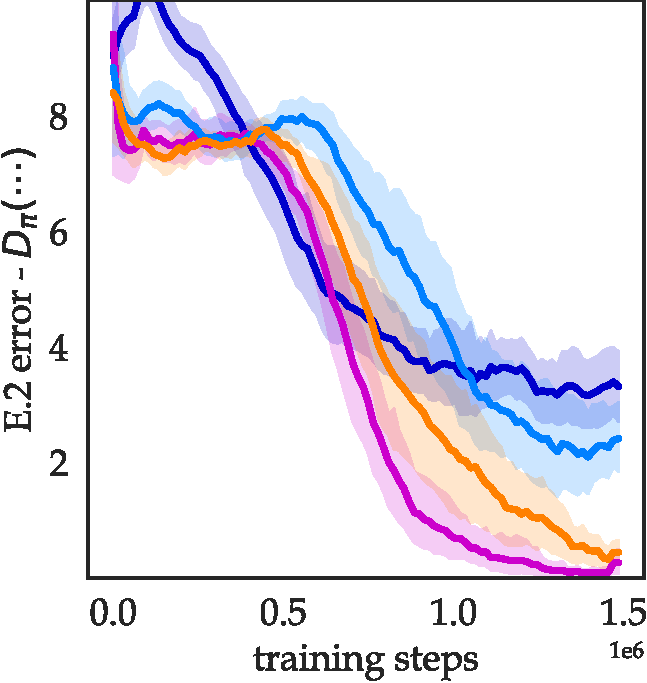
\includegraphics[height=0.31\textwidth]{figures/Delusions/fig_full_SSM_1.pdf}}
\hfill
\subfloat[\textit{Final \Ezero{} Errors by Distance}]{
\captionsetup{justification = centering}
\includegraphics[height=0.31\textwidth]{figures/Delusions/fig_full_SSM_5.pdf}}

\subfloat[\textit{Evolution of \Eone{} Behavior Ratio}]{
\captionsetup{justification = centering}
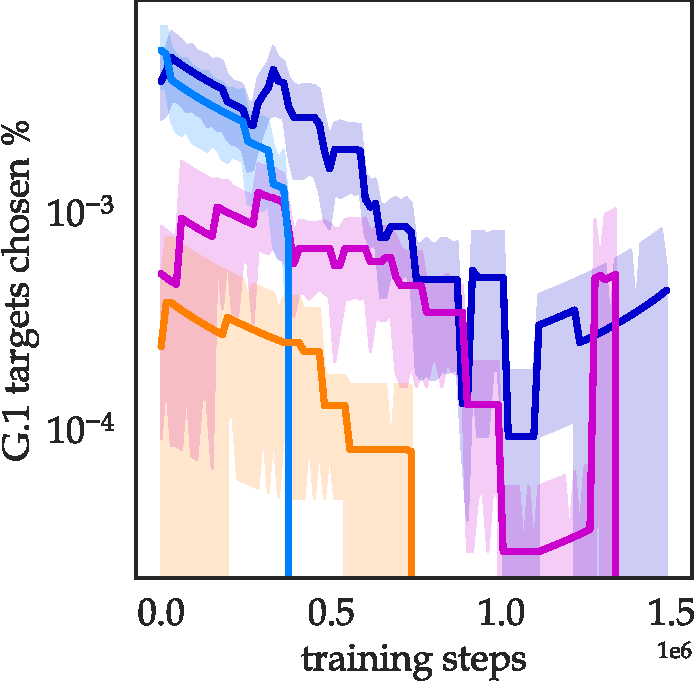
\includegraphics[height=0.31\textwidth]{figures/Delusions/fig_full_SSM_2.pdf}}
\hfill
\subfloat[\textit{Evolution of \Etwo{} Behavior Ratio}]{
\captionsetup{justification = centering}
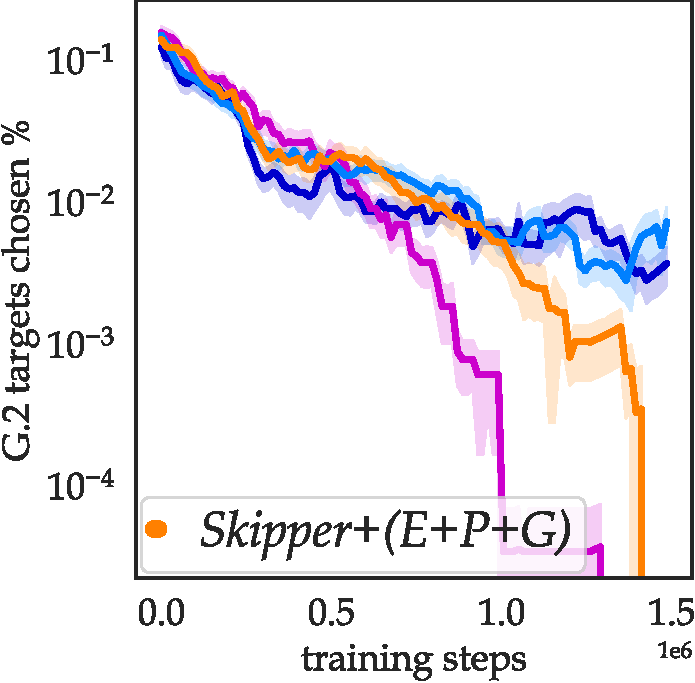
\includegraphics[height=0.31\textwidth]{figures/Delusions/fig_full_SSM_3.pdf}}
\hfill
\subfloat[\textit{Aggregated OOD Performance}]{
\captionsetup{justification = centering}
\includegraphics[height=0.31\textwidth]{figures/Delusions/fig_full_skipper_SSM_aggregate.pdf}}

\caption[Details of Skipper's Performance on SSM]{\textbf{Details of \Skipper{}'s Performance on \SSM{}}: All error bars (95\%-CI) are established over $20$ seed runs. We compare the original form of \Skipper{}, which learns its own feasibility estimates of target states in its own way, against three \Skipper{}+ variants, which have our proposed evaluator injected to assist the evaluation of the feasibility of targets, powered by the \FEG{}, \FEP{} \& \FEPG{} relabeling strategies, respectively. \textbf{a)}: Final \Ezero{} errors separated across a range of ground truth distances. Both estimated and true distances are conditioned on the evolving policies; \textbf{b)}: \Eone{} errors measured as $L_1$ error in estimated (clipped) distance throughout training; \textbf{c)}: \Gtwo{}-counterparts of \textbf{b}; \textbf{d)} \& \textbf{e)}: the changes of frequencies in delusional behaviors throughout training, for \Gone{} and \Gtwo{} composed targets, respectively. The curves denote the frequencies of \Gone{} and \Gtwo{} targets becoming the imminent subgoals that \Skipper{} seeks to achieve next; \textbf{f)}: Each data point represents OOD evaluation performance aggregated over $4 \times 20$ newly generated tasks, with mean difficulty matching training. The decomposed results for each OOD difficulty are presented in Fig.~\ref{fig:SSM_perfevol}.
}
\label{fig:Skipper_SSM}
\end{figure*}

We compare the original form of \Skipper{} with \SkipperPlus{}, a variant that is assisted by the proposed evaluator. Details of the variants are shown in the captions of Fig.~\ref{fig:Skipper_SSM}.

\phantomsection
\label{sec:hallucination_freqs}
\paragraph{Hallucination} We first investigate generator's rates of hallucinations. As shown in Fig.~\ref{fig:hallucination_frequencies}, the generator produces targets that correspond to \Gone{} and \Gtwo{} with the rate of around $3\%$ and $5\%$, respectively.

We use hindsight-relabeled transitions to train the generators in the two methods, to demonstrate how different ways of training the generator could affect the rates of hallucinations. \Gtwo{} can appear more frequently if the generator is trained to imagine more diverse kinds of targets than needed. For example, a conditional target generator which learns from \episodestr{} will be more likely to produce \Gtwo{} target states (compared to \futurestr{}). This was why we mostly used \futurestr{} to train the generators in the related experiments.

For the HER-trained generators, Fig.~\ref{fig:hallucination_frequencies} \textbf{a)}, shows that different training targets for the generator could lead to different degrees of hallucinations, in terms of \Gone{} and \Gtwo{}, but not $0$. Importantly, Fig.~\ref{fig:hallucination_frequencies} \textbf{b)} indicates that, \futurestr{} generates \Gtwo{} target states significantly less frequently than \episodestr{} and \pertaskstr{}, as the other two wasted training budget on \Gtwo{} target states, especially \pertaskstr{} that brings in more problematic training samples from long distances. \textit{In all other experiments, we only compare variants with \futurestr{} for the generator training.}

The generator is consistently used for both \Skipper{} and \LEAP{} in these 4 sets of experiments.

\begin{figure*}[htbp]
\centering

\subfloat[\textit{\Gone{} Candidate Ratio in \SSM{}}]{
\captionsetup{justification = centering}
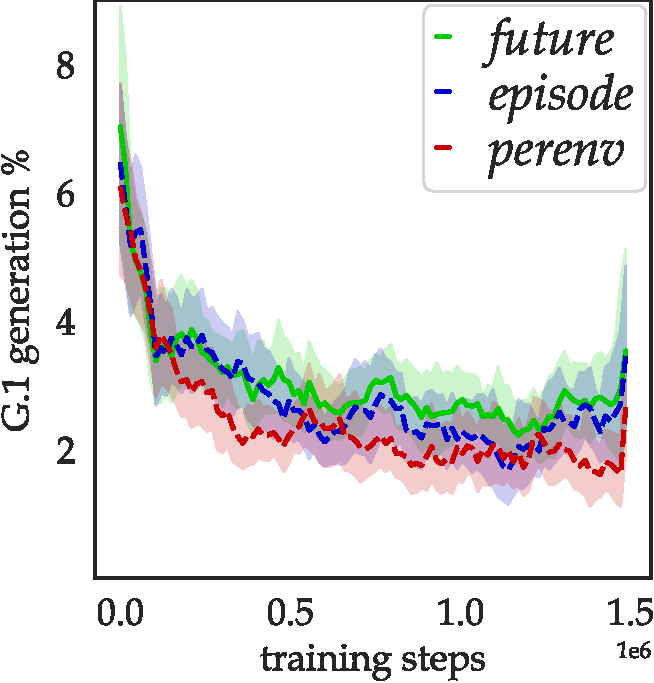
\includegraphics[height=0.32\textwidth]{figures/Delusions/fig_main_SSM_7.pdf}}
\hfill
\subfloat[\textit{\Gtwo{} Candidate Ratio in \SSM{}}]{
\captionsetup{justification = centering}
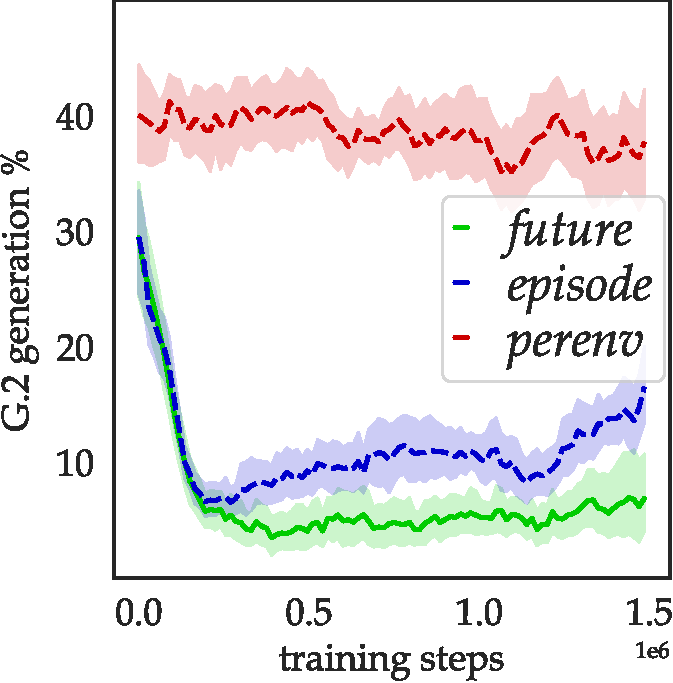
\includegraphics[height=0.32\textwidth]{figures/Delusions/fig_main_SSM_8.pdf}}
\hfill
\subfloat[\textit{\Gone{} Candidate Ratio in \RDS{}}]{
\captionsetup{justification = centering}
\includegraphics[height=0.32\textwidth]{figures/Delusions/fig_main_RDS_0.pdf}}

\caption[Hallucination Frequencies]{\textbf{Hallucination Frequencies}: All error bars (95\%-CI) are established over $20$ seed runs. \textbf{a)} Evolving ratio of \Gone{} ``states'' among all candidates at each target selection, throughout training; Subfigure \textbf{b)} is the \Etwo{}-counterpart of \textbf{a)} on \SSM{}; Subfigure \textbf{c)} is the \RDS{}-counterpart of \textbf{a)}.
}
\label{fig:hallucination_frequencies}
\end{figure*}

\paragraph{Feasibility Errors}
\Skipper{} relies on a built-in cumulative discount estimator whose estimations can be converted to feasibility estimates that our evaluator seeks to learn. Thus, we can examine the errors of the feasibility estimates corrected by the injected evaluator to understand how the proposed evaluator could reduce feasibility delusions of arbitrary-horizon TAP methods. From Fig.~\ref{fig:Skipper_SSM} \textbf{b}) and \textbf{c)}, we can see that feasibility estimates corrected by our evaluator have significantly less errors compared to the original, towards both \Gone{} and \Gtwo{} targets. As a perk for \SkipperPlus{}'s utilization of \pertaskstr{} for \Etwo{} delusions (included in \FEPG{}), its positive effect on far-away \Gzero{} targets are also shown in Fig.~\ref{fig:Skipper_SSM} \textbf{a)}. It can be seen that the evaluator is generally helpful for \Skipper{} to understand the feasibility of all \Gzero{}, \Gone{} and \Gtwo{} targets.

\paragraph{Frequency of Delusional Plans}
The purpose of identifying infeasible targets is to reduce delusional plans that involve them. We provide detailed results on this in Fig.~\ref{fig:Skipper_SSM}, where we observed significant reduction in delusional plans involving both \Gone{} and \Gtwo{} targets.

\paragraph{Generalization}
Comparing \Skipper{} and \SkipperPlus{}, we can deduce from Fig.~\ref{fig:Skipper_SSM} that generally, lower \Etwo{} errors (\textbf{c}) lead to less frequent delusional behaviors (\textbf{d} \& \textbf{e})), which in turn improves the OOD performance in \textbf{f)}. This indicates that rejecting infeasible targets can help decision-time TAP agents in systematic OOD generalization.

\paragraph{Breakdown of Task Performance}
In Fig.~\ref{fig:SSM_perfevol}, we present the evolution of \Skipper{} variants' performance on the training tasks as well as the OOD evaluation tasks throughout the training process. Note that Fig.~\ref{fig:Skipper_SSM} \textbf{h)} is an aggregation of all $4$ sources of OOD performance in Fig.~\ref{fig:SSM_perfevol} \textbf{b-e)}.

From the performance advantages of the hybrid variants (in both training and evaluation tasks), we can see that learning to address delusions during training brings better understanding for novel situations posed in OOD tasks.

\begin{figure}[htbp]
\centering

\subfloat[training, $\delta=0.4$]{
\captionsetup{justification = centering}
\includegraphics[height=0.22\textwidth]{figures/Delusions/fig_SSM_perfevol_0.pdf}}
\hfill
\subfloat[OOD evaluation, $\delta=0.25$]{
\captionsetup{justification = centering}
\includegraphics[height=0.22\textwidth]{figures/Delusions/fig_SSM_perfevol_1.pdf}}
\hfill
\subfloat[OOD evaluation, $\delta=0.35$]{
\captionsetup{justification = centering}
\includegraphics[height=0.22\textwidth]{figures/Delusions/fig_SSM_perfevol_2.pdf}}
\hfill
\subfloat[OOD evaluation, $\delta=0.45$]{
\captionsetup{justification = centering}
\includegraphics[height=0.22\textwidth]{figures/Delusions/fig_SSM_perfevol_3.pdf}}
\hfill
\subfloat[OOD evaluation, $\delta=0.55$]{
\captionsetup{justification = centering}
\includegraphics[height=0.22\textwidth]{figures/Delusions/fig_SSM_perfevol_4.pdf}}
\caption[Evolution of OOD Performance of \Skipper{} Variants on \SSM{}]{\textbf{Evolution of OOD Performance of \Skipper{} Variants on \SSM{}}: All error bars (95\%-CI) are established over $20$ seed runs. 
}
\label{fig:SSM_perfevol}
\end{figure}

\subsubsection{\LEAP{} on \SSM{} \texorpdfstring{(Exp.~$\nicefrac{2}{8}$)}{(Exp.~2/8)}}
This set of experiments seeks to demonstrate that the proposed feasibility evaluator is applicable to other decision-time TAP agents, utilizing their generators in different ways. For this purpose, we study \LEAP{} performance on \SSM{}, with or without the help of the target rejection provided by the feasibility estimators.

\LEAP{} is different from \Skipper{}, as its decision-time planning process constructs a singular sequence of subgoals leading to the task goal. Due to a lack of backup subgoals, even if one among them is problematic, the whole resulting plan would be delusional, making \LEAP{} much more prone to failures compared to \Skipper{}, where candidate targets can still be reused if deviation from the original plan occurred.

\SSM{} has a relatively large state space that requires more intermediate subgoals for \LEAP{}'s plans. However, an increment of the number of subgoals also dramatically increases the frequencies of delusional plans, damaging the agents' performance. Because of this, our experimental results of \LEAP{} on \SSM{} with size $12 \times 12$ became difficult to analyze because of the rampant failures. We chose instead to present the results on \SSM{} with size $8 \times 8$ here.

\begin{figure*}[htbp]
\centering

\subfloat[\textit{\Gone{} Ratio Planned}]{
\captionsetup{justification = centering}
\includegraphics[height=0.19\textwidth]{figures/Delusions/fig_LEAP_SSM_8x8_0.pdf}}
\hfill
\subfloat[\textit{\Gtwo{} Ratio Planned}]{
\captionsetup{justification = centering}
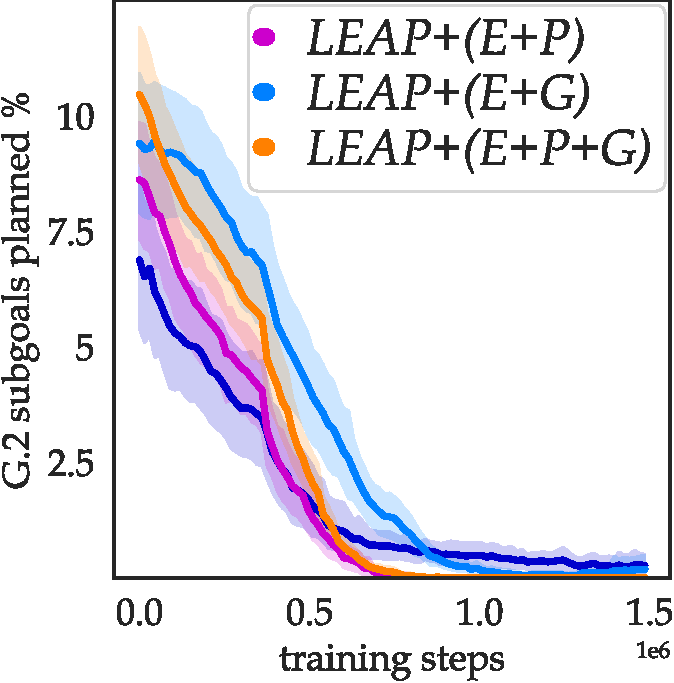
\includegraphics[height=0.19\textwidth]{figures/Delusions/fig_LEAP_SSM_8x8_1.pdf}}
\hfill
\subfloat[\textit{Delusional Plan Ratio}]{
\captionsetup{justification = centering}
\includegraphics[height=0.19\textwidth]{figures/Delusions/fig_LEAP_SSM_8x8_2.pdf}}
\hfill
\subfloat[\textit{\Ezero{} Errors}]{
\captionsetup{justification = centering}
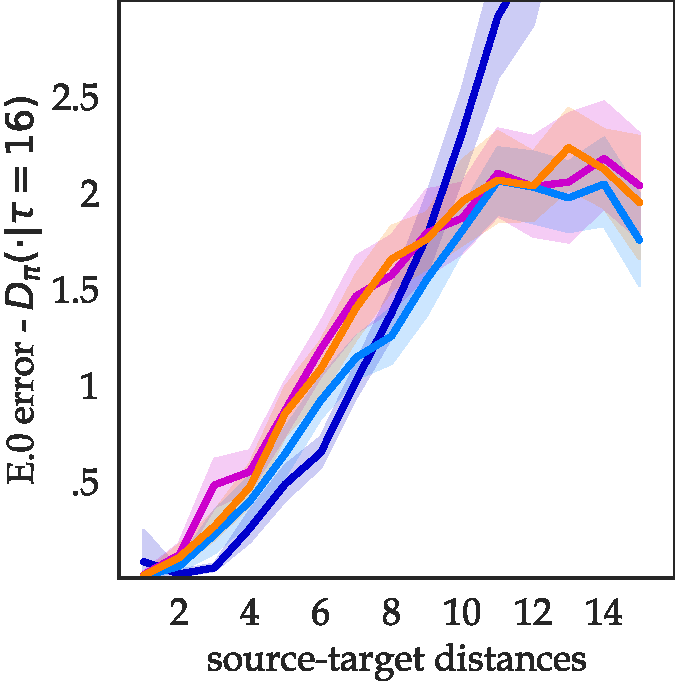
\includegraphics[height=0.19\textwidth]{figures/Delusions/fig_LEAP_SSM_8x8_3.pdf}}
\hfill
\subfloat[\textit{Aggregated OOD Perf.}]{
\captionsetup{justification = centering}
\includegraphics[height=0.19\textwidth]{figures/Delusions/fig_LEAP_SSM_8x8_4.pdf}}

\caption[LEAP on SSM]{\textbf{\LEAP{} on \SSM{}}: All error bars (95\%-CI) are established over $20$ seed runs. \textbf{a)} Ratio of \Gone{} subgoals among the planned sequences; \textbf{b)} Ratio of \Gtwo{} subgoals in the planned sequences; \textbf{c)} Ratio of evolved sequences containing at least one \Gone{} or \Gtwo{} target; \textbf{d)} The final estimation accuracies towards \Gzero{} targets after training completed, across a spectrum of ground truth distances. In this figure, both distances (estimation and ground truth) are conditioned on the final version of the evolving policies; \textbf{e)} Each data point represents OOD evaluation performance aggregated over $4 \times 20$ newly generated tasks, with mean difficulty matching the training tasks.
}

\label{fig:LEAP_SSM}
\end{figure*}

For \LEAP{}, we use some different metrics to analyze the effectiveness of the proposed strategies in addressing delusions. This is because, if \LEAP{}'s evaluator successfully addressed delusions and learned not to favor the problematic targets (\Gone{} and \Gtwo{}), then they will not be selected in the evolved elitist sequence of subgoals. This makes it inconvenient for us to use the distance error in the delusional source-target pairs during decision-time as a metric to analyze the reduction of delusional estimates, because of their growing scarcity.

As we can see from Fig. \ref{fig:LEAP_SSM}, similar arguments about the effectiveness of the proposed hybrid strategies can be made, to those with \Skipper{}. The hybrids with more investment in addressing \Eone{}, \ie{}, \FEG{} and \FEPG{}, exhibit the lowest \Eone{} errors (\textbf{a)}). Similarly, \FEP{} and \FEPG{} achieve the lowest \Etwo{} errors (\textbf{b)}). In \textbf{e)}, we see that the $3$ hybrid variants achieve better OOD performance than the baseline \FE{}. Specifically, \FEG{} achieved the best performance. This is likely because that it induced the highest sample efficiency in terms of learning the estimations towards \Gzero{} subgoals, as shown in \textbf{d)}. Assistive strategies such as \generatestr{} and \pertaskstr{} do not only induce problematic targets, but also \Gzero{} ones that can shift the training distribution towards higher sample efficiencies in the traditional sense.

\paragraph{Breakdown of Task Performance}
In Fig. \ref{fig:LEAP_SSM_perfevol}, we present the evolution of \LEAP{} variants' performance on the training tasks as well as the OOD evaluation tasks throughout the training process. Note that Fig. \ref{fig:LEAP_SSM} \textbf{e)} is an aggregation of all $4$ sources of OOD performance in Fig. \ref{fig:LEAP_SSM_perfevol} \textbf{b-e)}.

\begin{figure*}[htbp]
\centering

\subfloat[training, $\delta=0.4$]{
\captionsetup{justification = centering}
\includegraphics[height=0.22\textwidth]{figures/Delusions/fig_LEAP_SSM_8x8_perfevol_0.pdf}}
\hfill
\subfloat[OOD evaluation, $\delta=0.25$]{
\captionsetup{justification = centering}
\includegraphics[height=0.22\textwidth]{figures/Delusions/fig_LEAP_SSM_8x8_perfevol_1.pdf}}
\hfill
\subfloat[OOD evaluation, $\delta=0.35$]{
\captionsetup{justification = centering}
\includegraphics[height=0.22\textwidth]{figures/Delusions/fig_LEAP_SSM_8x8_perfevol_2.pdf}}
\hfill
\subfloat[OOD evaluation, $\delta=0.45$]{
\captionsetup{justification = centering}
\includegraphics[height=0.22\textwidth]{figures/Delusions/fig_LEAP_SSM_8x8_perfevol_3.pdf}}
\hfill
\subfloat[OOD evaluation, $\delta=0.55$]{
\captionsetup{justification = centering}
\includegraphics[height=0.22\textwidth]{figures/Delusions/fig_LEAP_SSM_8x8_perfevol_4.pdf}}

\caption[Evolution of OOD Performance of LEAP Variants on SSM]{\textbf{Evolution of OOD Performance of \LEAP{} Variants on \SSM{}}: All error bars (95\%-CI) are established over $20$ seed runs. 
}

\label{fig:LEAP_SSM_perfevol}
\end{figure*}

\subsubsection{\Skipper{} on \RDS{} \texorpdfstring{(Exp.~$\nicefrac{3}{8}$)}{(Exp.~3/8)}}

This set of experiments focus on the feasibility evaluator's abilities in the face of \Gone{} challenges. We present \Skipper{}'s evaluative curves in Fig. \ref{fig:main_RDS}.

\begin{figure*}[htbp]
\centering

\subfloat[\textit{\Eone{} Estimation Errors}]{
\captionsetup{justification = centering}
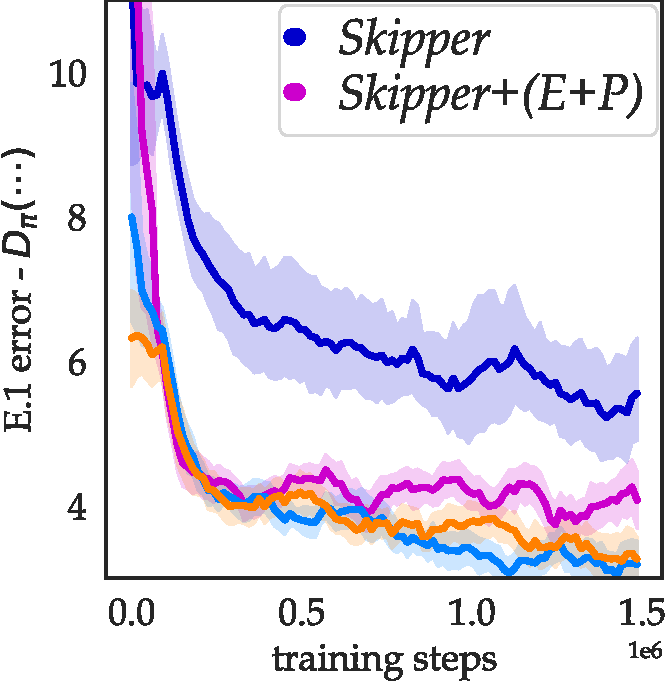
\includegraphics[height=0.24\textwidth]{figures/Delusions/fig_full_RDS_1.pdf}}
\hfill
\subfloat[\textit{\Gone{} + \Eone{} Behavior Ratio}]{
\captionsetup{justification = centering}
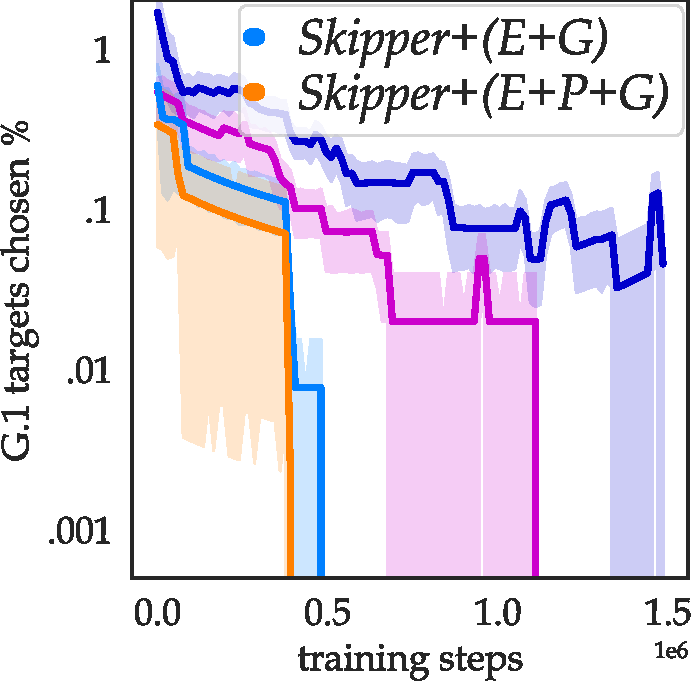
\includegraphics[height=0.24\textwidth]{figures/Delusions/fig_full_RDS_2.pdf}}
\hfill
\subfloat[\textit{\Ezero{} Errors}]{
\captionsetup{justification = centering}
\includegraphics[height=0.24\textwidth]{figures/Delusions/fig_full_RDS_3.pdf}}
\hfill
\subfloat[\textit{Aggregated OOD Perf.}]{
\captionsetup{justification = centering}
\includegraphics[height=0.24\textwidth]{figures/Delusions/fig_full_RDS_4.pdf}}

\caption[Skipper's Performance on RDS]{\textbf{\Skipper{}'s Performance on \RDS{}}: All error bars (95\%-CI) are established over $20$ seed runs. \textbf{a)} \Eone{} delusions in terms of $L_1$ error in estimated distance is visualized, throughout the training process. \textbf{b)} The curves represent the frequencies of choosing \Gone{} ``states'' whenever a selection of targets is initiated; \textbf{c)} The final estimation accuracies towards \Gzero{} target states after training completed, across a spectrum of ground truth distances. In this figure, both distances (estimation and ground truth) are conditioned on the final version of the evolving policies; The state structure of \RDS{} does not allow \Gtwo{} target states and the corresponding \Etwo{} delusions; \textbf{d)} Each data point represents OOD evaluation performance aggregated over $4 \times 20$ newly generated tasks, with mean difficulty matching the training tasks.
}

\label{fig:main_RDS}
\end{figure*}

From Fig. \ref{fig:main_RDS} \textbf{d)}, we can see that, probably because of the lack of dominant \Gtwo{} + \Etwo{} cases, the OOD performance of even the most basic \episodestr{} variant is high, despite the hybrid variants perform even better. \FEG{}, \ie{} the hybrid with the most investment in \generatestr{} (aiming at \Eone{}), performs the best both in terms of \Eone{} delusion suppression (\textbf{a)}), and OOD generalization (\textbf{d)}), as expected. In \RDS{}, the short-distance \Ezero{} estimation accuracy as well as the OOD performance of \FP{} are not as bad as in \SSM{}. This is possibly because \RDS{} has much smaller state spaces, where \episodestr{} and \pertaskstr{} produce more similar results (than in large state spaces of \SSM{}).

\paragraph{Breakdown of Task Performance}
In Fig. \ref{fig:RDS_perfevol}, we present the evolution of \Skipper{} variants' performance on the training tasks as well as the OOD evaluation tasks throughout the training process. Note that Fig. \ref{fig:main_RDS} \textbf{d)} is an aggregation of all $4$ sources of OOD performance in Fig. \ref{fig:RDS_perfevol} \textbf{b-e)}.

\begin{figure*}[htbp]
\centering

\subfloat[training, $\delta=0.4$]{
\captionsetup{justification = centering}
\includegraphics[height=0.22\textwidth]{figures/Delusions/fig_RDS_perfevol_0.pdf}}
\hfill
\subfloat[OOD evaluation, $\delta=0.25$]{
\captionsetup{justification = centering}
\includegraphics[height=0.22\textwidth]{figures/Delusions/fig_RDS_perfevol_1.pdf}}
\hfill
\subfloat[OOD evaluation, $\delta=0.35$]{
\captionsetup{justification = centering}
\includegraphics[height=0.22\textwidth]{figures/Delusions/fig_RDS_perfevol_2.pdf}}
\hfill
\subfloat[OOD evaluation, $\delta=0.45$]{
\captionsetup{justification = centering}
\includegraphics[height=0.22\textwidth]{figures/Delusions/fig_RDS_perfevol_3.pdf}}
\hfill
\subfloat[OOD evaluation, $\delta=0.55$]{
\captionsetup{justification = centering}
\includegraphics[height=0.22\textwidth]{figures/Delusions/fig_RDS_perfevol_4.pdf}}

\caption[Evolution of OOD Performance of Skipper Variants on RDS]{\textbf{Evolution of OOD Performance of \Skipper{} Variants on \RDS{}}: All error bars (95\%-CI) are established over $20$ seed runs.
}

\label{fig:RDS_perfevol}
\end{figure*}

\subsubsection{\LEAP{} on \RDS{} \texorpdfstring{(Exp.~$\nicefrac{4}{8}$)}{(Exp.~4/8)}}

This set of experiments focus on \LEAP{}'s performance on \RDS{}. Similarly, we present the evaluative metrics in Fig. \ref{fig:LEAP_RDS}.

\begin{figure*}[htbp]
\centering

\subfloat[\textit{\Gone{} Ratio in Planned Sequence}]{
\captionsetup{justification = centering}
\includegraphics[height=0.24\textwidth]{figures/Delusions/fig_full_LEAP_RDS_0.pdf}}
\hfill
\subfloat[\textit{Delusional Plan Ratio}]{
\captionsetup{justification = centering}
\includegraphics[height=0.24\textwidth]{figures/Delusions/fig_full_LEAP_RDS_1.pdf}}
\hfill
\subfloat[\textit{\Ezero{} Estim. Errors}]{
\captionsetup{justification = centering}
\includegraphics[height=0.24\textwidth]{figures/Delusions/fig_full_LEAP_RDS_2.pdf}}
\hfill
\subfloat[\textit{Aggregated OOD Performance}]{
\captionsetup{justification = centering}
\includegraphics[height=0.24\textwidth]{figures/Delusions/fig_full_LEAP_RDS_3.pdf}}

\caption[LEAP's Performance on RDS]{\textbf{\LEAP{}'s Performance on \RDS{}}: All error bars (95\%-CI) are established over $20$ seed runs. \textbf{a)} Ratio of \Gone{} subgoals among the planned sequences; \textbf{b)} Ratio of planned sequences containing at least one \Gone{} target; \textbf{c)} The final estimation accuracies towards \Gzero{} target states after training completed, across a range of ground truth distances. In this figure, both distances (estimation and ground truth) are conditioned on the final version of the learned policies; \textbf{d)} Each data point represents OOD evaluation performance aggregated over $4 \times 20$ newly generated tasks, with mean difficulty matching the training tasks.
}
\label{fig:LEAP_RDS}
\end{figure*}

The conclusions are similar, despite that the OOD performance gain by addressing delusions is significantly higher than in \SSM{}.

\paragraph{Breakdown of Task Performance}
In Fig. \ref{fig:LEAP_RDS_perfevol}, we present the evolution of \LEAP{} variants' performance on the training tasks as well as the OOD evaluation tasks throughout the training process. Note that Fig. \ref{fig:LEAP_RDS} \textbf{d)} is an aggregation of all $4$ sources of OOD performance in Fig. \ref{fig:LEAP_RDS_perfevol} \textbf{b-e)}.

\begin{figure*}[htbp]
\centering

\subfloat[training, $\delta=0.4$]{
\captionsetup{justification = centering}
\includegraphics[height=0.22\textwidth]{figures/Delusions/fig_LEAP_RDS_perfevol_0.pdf}}
\hfill
\subfloat[OOD evaluation, $\delta=0.25$]{
\captionsetup{justification = centering}
\includegraphics[height=0.22\textwidth]{figures/Delusions/fig_LEAP_RDS_perfevol_1.pdf}}
\hfill
\subfloat[OOD evaluation, $\delta=0.35$]{
\captionsetup{justification = centering}
\includegraphics[height=0.22\textwidth]{figures/Delusions/fig_LEAP_RDS_perfevol_2.pdf}}
\hfill
\subfloat[OOD evaluation, $\delta=0.45$]{
\captionsetup{justification = centering}
\includegraphics[height=0.22\textwidth]{figures/Delusions/fig_LEAP_RDS_perfevol_3.pdf}}
\hfill
\subfloat[OOD evaluation, $\delta=0.55$]{
\captionsetup{justification = centering}
\includegraphics[height=0.22\textwidth]{figures/Delusions/fig_LEAP_RDS_perfevol_4.pdf}}

\caption[Evolution of OOD Performance of LEAP Variants on RDS]{\textbf{Evolution of OOD Performance of \LEAP{} Variants on \RDS{}}: All error bars (95\%-CI) are established over $20$ seed runs.
}

\label{fig:LEAP_RDS_perfevol}
\end{figure*}


\begin{figure}[htbp]
\centering

\subfloat[\textit{Convergence to Optimal Value}]{
\captionsetup{justification = centering}
\includegraphics[height=0.32\textwidth]{figures/Delusions/fig_Dyna_SSM_0.pdf}}
\hfill
\subfloat[\textit{Training Performance}]{
\captionsetup{justification = centering}
\includegraphics[height=0.32\textwidth]{figures/Delusions/fig_Dyna_SSM_1.pdf}}

\caption[Dyna's Performance on SSM]{\textbf{\Dyna{}'s Performance on \SSM{}}: All error bars (95\%-CI) are established over $20$ seed runs. Compared to the baseline \Dyna{}, \DynaPlus{} rejects the updates toward $1$-infeasible generated states flagged by the evaluator, powered by \FEPG{}. \textbf{a)} Evolving mean $L_1$ distances between estimated $Q$ \& optimal values; \textbf{b)}: task performance on the $50$ training tasks \& \textcolor{purple}{rate of \DynaPlus{} rejecting updates}.
}
\label{fig:Dyna_SSM}
\end{figure}


\subsection{Rejecting Destabilizing Updates in Background Planning (Exp.~$\nicefrac{5}{8}$ - Exp.~$\nicefrac{6}{8}$)}
\label{sec:exp_main_dyna}

For background planning agents, since they are by design not as good as decision-time planning agents in OOD generalization, we only compare the difference in their training performance.

These two sets of experiments focus on a rollout-based background TAP agent - the classical 1-step \Dyna{} \citep{sutton1991dyna}, which uses its learned transition model to generate next states from existing states to construct simulated transitions that are used to update the value estimator, \ie{} a ``\Dyna{} update''. \citet{jafferjee2020hallucinating} demonstrated the benefit when the delusional \Dyna{} updates bootstrapped on hallucinated targets are rejected with an oracle. We replace the oracle using our learned evaluator.


With the same training setup, in Fig.~\ref{fig:Dyna_SSM}, we present the empirical results of how target rejection can significantly improve the performance of \Dyna{} on \SSM{}. The rejection rate stabilizes as both the generator and the evaluator learns. These observations are consistent with Exp.~$\nicefrac{6}{8}$, presented in Sec.~\ref{sec:exp_RDS_dyna}.\footnote{The implementation here can be extended to fixed-horizon rollout agents. In the Sec.~\ref{sec:appendix_dreamer}, we provide details on how we applied our \Dyna{} solution to \Dreamer{}V2 \citep{hafner2020mastering}.}

% \subsection{Background Planning: \texorpdfstring{\Dyna{} on \RDS{} (Exp.~$\nicefrac{6}{8}$)}{Dyna on RDS (Exp.~6/8)}}
\phantomsection
\label{sec:exp_RDS_dyna}

In Fig.~\ref{fig:Dyna_RDS}, we present the empirical performance of a \Dyna{} variant with rejection enabled by \FEPG{}, which is significantly better than the baseline.

\begin{figure*}[htbp]
\centering

\subfloat[\textit{Convergence to Optimal Value}]{
\captionsetup{justification = centering}
\includegraphics[height=0.32\textwidth]{figures/Delusions/fig_Dyna_RDS_0.pdf}}
\hfill
\subfloat[\textit{Training Performance}]{
\captionsetup{justification = centering}
\includegraphics[height=0.32\textwidth]{figures/Delusions/fig_Dyna_RDS_1.pdf}}
\hfill
\subfloat[\textit{Training Performance}]{
\captionsetup{justification = centering}
\includegraphics[height=0.32\textwidth]{figures/Delusions/fig_Dyna_RDS_2.pdf}}

\caption[Dyna's Performance on RDS]{\textbf{\Dyna{}'s Performance on \RDS{}}: All error bars (95\%-CI) are established over $20$ seed runs. \textbf{a)}: Evolving mean $L_1$ distances between estimated $Q$ values \& ground truth optimals; \textbf{b)}: evaluation performance on the $50$ training tasks; \textbf{c)}: \textcolor{purple}{rate of rejecting \Dyna{} updates}.
}
\label{fig:Dyna_RDS}
\end{figure*}

\subsection{Feasibility Convergence to Non-Singleton Targets \texorpdfstring{(Exp.~$\nicefrac{7}{8}$ \& $\nicefrac{8}{8}$)}{(Exp.~7/8 \& Exp.~8/8)}}
We test if our implemented feasibility evaluator for Exp.~$\nicefrac{1}{8}$ - Exp.~$\nicefrac{4}{8}$ could withstand targets that are non-singleton. In its previous implementation, we use $h$ to enforce the that the targets are singletons. In fact, each $\bm{g}^\odot$ takes the form of a state representation and $h$ is only activated if a state with exactly the same representation is reached. For the non-singleton experiments however, we let $h$ activate when a state is within distance one to the target state, effectively expanding each target set from size $1$ to maximally size $5$. Given the new termination mechanisms enforced by the new $h$, each target now, despite still taking the form of a state representation, has a new meaning. This setting mirrors the goal-conditioned path planning agents that seeks to reach certain neighborhoods of the planned waypoints.

With this setting, we can also intuitively analyze the composition of the target set. Specifically, if one of the member state is \Gtwo{}, then the whole target set are fully made of \Gtwo{}. If all the $5$ states are out of the state space, then the target is fully composed of \Gone{}. For \SSM{}, a target in the temporarily unreachable situation, \eg{}, $s \in \langle 1, 1 \rangle$ with target encoding $s^\odot \in \langle 0, 1 \rangle $, could be composed of not only \Gtwo{} states but also some \Gone{}.

We apply the new $h$ to evaluator training and to the ground truth DP solver, and then compare their differences. As we could observe from Fig.~\ref{fig:nonsingleton_SSM}, the proposed feasibility evaluator, with the help of the two assistive hindsight relabeling strategy, significantly reduces the feasibility errors in all categories.

\begin{figure*}[htbp]
\centering

\subfloat[\textit{Evolution of \Ezero{} Errors}]{
\captionsetup{justification = centering}
\includegraphics[height=0.31\textwidth]{figures/Delusions/fig_nonsingleton_SSM_0.pdf}}
\hfill
\subfloat[\textit{Evolution of \Eone{} Errors}]{
\captionsetup{justification = centering}
\includegraphics[height=0.31\textwidth]{figures/Delusions/fig_nonsingleton_SSM_1.pdf}}
\hfill
\subfloat[\textit{Evolution of \Etwo{} Errors}]{
\captionsetup{justification = centering}
\includegraphics[height=0.31\textwidth]{figures/Delusions/fig_nonsingleton_SSM_2.pdf}}

\caption[Feasibility of Non-Singleton Targets on SSM]{\textbf{Feasibility of Non-Singleton Targets on \SSM{}}: All error bars (95\%-CI) are established over $20$ seed runs. \textbf{a)} Evolution of \Ezero{} error; \textbf{b)} Evolution of \Eone{} error; \textbf{c)} Evolution of \Etwo{} error; The training data is acquired with random walk, since the introduced non-singleton targets do not lead to adequate performances.
}

\label{fig:nonsingleton_SSM}
\end{figure*}


We observe the similar results in \RDS{}, presented in Fig.~\ref{fig:nonsingleton_RDS}.

\begin{figure*}[htbp]
\centering

\subfloat[\textit{Evolution of \Ezero{} Errors}]{
\captionsetup{justification = centering}
\includegraphics[height=0.32\textwidth]{figures/Delusions/fig_nonsingleton_RDS_0.pdf}}
\hfill
\subfloat[\textit{Evolution of \Eone{} Errors}]{
\captionsetup{justification = centering}
\includegraphics[height=0.32\textwidth]{figures/Delusions/fig_nonsingleton_RDS_1.pdf}}

\caption[Feasibility of Non-Singleton Targets on RDS]{\textbf{Feasibility of Non-Singleton Targets on \RDS{}}: All error bars (95\%-CI) are established over $20$ seed runs. \textbf{a)} Evolution of \Ezero{} error; \textbf{b)} Evolution of \Eone{} error; The training data is acquired with random walk, since the introduced non-singleton targets do not lead to adequate performances.
}

\label{fig:nonsingleton_RDS}
\end{figure*}

\section{Summary}

We characterized how generator hallucinations can cause trouble for TAP agents. Then, we proposed to evaluate the feasibility of targets \st{} the infeasible hallucinations can be properly rejected during planning. We proposed a combination of learning rules, architectures and data augmentation strategies that leads to robust and accurate output when the proposed evaluator is applied. In experiments, we showed that the evaluator can significantly address the harm of hallucinated targets in various kinds of planning agents. 
